\documentclass[12pt,a4paper,oneside]{report}
\usepackage[utf8]{inputenc}

\usepackage{enumerate}
\usepackage{amsmath}
\usepackage{amssymb}
\usepackage{graphicx}
\usepackage{subfigure}
\usepackage[left=3cm,right=3cm,top=3cm,bottom=4cm]{geometry}
\usepackage{caption}
\usepackage{indentfirst}
\usepackage{multirow}
\usepackage{titlesec}
\usepackage{indentfirst}
\usepackage{cite}
\usepackage{algorithm}  
\usepackage{algorithmicx}  
\usepackage{algpseudocode}
\usepackage{tikz}

\renewcommand{\algorithmicrequire}{\textbf{Input:}}  
\renewcommand{\algorithmicensure}{\textbf{Output:}}  


\renewcommand{\thechapter}{\Roman{chapter}}
\titleformat{\chapter}{\Huge\bfseries}{\thechapter}{0.5em}{}
\renewcommand{\thesection}{  \arabic{section}}


\author{
    \textbf{Joint Authors:}\\
    Gu Yichen 5143709162\\
    Lars Vagnes 5143709\\ 
    Liu Yihao 515370910207\\
    Zhu Yifan 5143709016\\
    \normalsize{(In Alphabetic Order)}\\
    \\
    \textbf{Instructor:}\\
    Prof. Charlemagne Manuel\\ \\ \textbf{Course:}\\VE475\\ Introduction to Cryptography\\ \\ \textbf{Institute:}\\University of Michigan - Shanghai Jiao Tong University\\Joint Institute}
\title{\textbf{Project:\\Message Authentication Code}}

\date{2017-July-1st}

\begin{document}
\maketitle

\begin{abstract}

\noindent \\
\end{abstract}


\tableofcontents
\chapter{  Introduction}
\section{Introduction to Cryptography}
The Concise Oxford Dictionary (2006) defines cryptography as the art of writing or solving codes.$^{[2]}$ However, in the late $20^{th}$ century, this picture of cryptography radically changed. A rich theory emerged, enabling the rigorous study of cryptography as a science. Cryptography is now about constructing and analyzing protocols that prevent third parties or the public from reading private messages.$^{[3]}$

\subsection{Classic Cryptography}
The main classical cipher types are transposition ciphers, which rearrange the order of letters in a message and substitution ciphers, which systematically replace letters or groups of letters with other letters or groups of letters. 

The earliest known use of cryptography is some carved ciphertext on stone in Egypt (ca 1900 BCE), but this may have been done for the amusement of literate observers rather than as a way of concealing information.

\subsection{Modern Cryptography}
Modern cryptography includes various aspects in information security such as data confidentiality, data integrity, authentication, and non-repudiation.$^{[4]}$ Applications of modern cryptography exist at the intersection of the disciplines of mathematics, computer science, and electrical engineering.

Here are several chief topics of modern cryptography:

\begin{itemize}
    \item \textbf{Symmetric-key cryptography}
    \item \textbf{Public-key cryptography}
    \item \textbf{Cryptanalysis}
    \item \textbf{Cryptographic primitives}
    \item \textbf{Cryptosystems}
\end{itemize}

\section{Introduction to Message Authentication}
Message authentication is a mechanism or service used to verify the integrity of a message. Message authentication assures that data received contain no modification, insertion, deletion, or replay and that the purported identity of the sender is valid.$^{[5]}$ 



\subsection{Message Authentication Functions}
Message authentication does not necessarily include the property of non-repudiation.$^{[6][7]}$ and is typically achieved by using message authentication codes (MACs), message encryption (ME) or hash function$^{[5]}$.

\begin{enumerate}[(1)]
    \item \textbf{Hash function:} A function that maps a message of any length into a fixed-length
hash value, which serves as the authenticator
    \item \textbf{Message encryption:} The ciphertext of the entire message serves as its authenticator
    \item \textbf{Message authentication code (MAC):} A function of the message and a secret
key that produces a fixed-length value that serves as the authenticator
\end{enumerate}

\subsection{Message Authentication Requirements}
In the context of communications across a network, message authentication can deal with the following four attacks.

\begin{enumerate}[(1)]
    \item \textbf{Masquerade:} Insertion of messages into the network from a fraudulent source.
    \item \textbf{Content modification:} Changes to the contents of a message.
    \item \textbf{Sequence modification:} Any modification to a sequence of messages between
parties.
    \item \textbf{Timing modification:} Delay or replay of messages.
\end{enumerate}

In summary, message authentication is a procedure to verify that received messages come from the alleged source and have not been altered. Message authentication may also verify sequencing and timeliness.$^{[5]}$
\\

However, there are still a few attacks that message authentication can not deal with. The following are some:

\begin{enumerate}[(1)]
    \item \textbf{Disclosure:} Release of message contents to any person or process not possessing the appropriate cryptographic key.
    \item \textbf{Traffic analysis:} Discovery of the pattern of traffic between parties.
    \item \textbf{Source repudiation:} Denial of transmission of message by source.
    \item \textbf{Destination repudiation} Denial of receipt of message by destination.
\end{enumerate}

Measures to deal with the first two attacks are in the realm of message confidentiality and are dealt with in Part One. Mechanisms for dealing specifically with item (3) come under the heading of digital signatures. A digital signature is an
authentication technique that also includes measures to counter repudiation by the source. Dealing with item (4) may require a combination of the use of digital signatures and a protocol designed to counter this attack.


\section{Introduction to Message Authentication Codes}
A message authentication code (MAC) is an algorithm that takes a variable-length message and a secret key as input and produces an authentication code. A recipient in possession of the secret key can generate an authentication code to verify the integrity of the message.$^{[]}$

There are two means of forming a MAC. One is to combine a cryptographic hash table in some fashion with a secret key. Another is to use a symmetric block cipher in such a way that it produces a fixed-length output for a variable-length input.

\subsection{Requirements for Message Authentication Codes}
Assume that an opponent knows the MAC function but does not know . Then the MAC function should satisfy the following requirements.

\begin{enumerate}
    \item If an opponent observes $M$ and MAC$(K,M)$, it should be computationally infeasible for the opponent to construct a message $M'$ such that
    $$MAC(K,M') = MAC(K,M)$$
    \item MAC$(K,M)$ should be uniformly distributed in the sense that for randomly chosen messages, $M$ and $M'$, the probability that $MAC(K,M') = MAC(K,M)$ is $2^{-n}$, where $n$ is the number of bits in the tag.
    \item Let $M'$ be equal to some known transformation on $M$.That is, $M'=f(M)$. For example, f may involve inverting one or more specific bits. In that case,
    $$Pr[MAC(K,M)=MAC(K,M')] = 2^{-n}$$
\end{enumerate}

The first requirement speaks to the example, in which an opponent is able to construct a new message to match a given tag, even though the opponent does not know and does not learn the key.

The second requirement deals with the need to thwart a brute-force attack based on chosen plaintext.

The final requirement dictates that the authentication algorithm should not be weaker with respect to certain parts or bits of the message than others.$^{[5]}$

\chapter{  MAC Classification}
\section{MAC Based on Block Ciphers}
\subsection{Definition of DAA}

The Data Authentication Algorithm (DAA) is based on DES, and it has been one of the most widely used MACs for a number of years. \\

The algorithm can be defined as using the cipher block chaining (CBC) mode of operation of DES with an initialization vector of zero. The data  to be authenticated are grouped into contiguous 64-bit
blocks: $D_1$, $D_2$, \dots, $D_n$. If necessary, the final block is padded on the right with zeroes
to form a full 64-bit block. Using the DES encryption algorithm E and a secret key $K$,
a data authentication code (DAC) is calculated as follows

\begin{align*}
    O_1 &= E(K,D_1) \\
    O_2 &= E(K,D_2 \oplus O_1) \\
    O_3 &= E(K,D_3 \oplus O_2) \\
    \vdots \\
    O_n &= E(K,D_n \oplus O_{n-1}) \\
\end{align*}

And then $O_n$ is the MAC of the data.\\

However, only messages of one fixed length of $mn$ bits
are processed, where $n$ is the cipher block size and $m$ is a fixed positive integer. As a
simple example, notice that given the CBC MAC of a one-block message $X$, say
$T = MAC(K, X)$, the adversary immediately knows the CBC MAC for the two-
block message $X \mid\mid (X \oplus T)$ since this is once again $T$.

\subsection{Definition of CMAC}

Black and Rogaway [BLAC00] demonstrated that the limitation of DAA could be
overcome using three keys: one key of length $K$ to be used at each step of the
cipher block chaining and two keys of length $n$, where $k$ is the key length and n is
the cipher block length. This proposed construction was refined by Iwata and
Kurosawa so that the two n-bit keys could be derived from the encryption key,
rather than being provided separately [IWAT03]. This refinement, adopted by
NIST, is the Cipher-based Message Authentication Code (CMAC) mode of operation
for use with AES and triple DES. \\

First, let us define the operation of CMAC when the message is an integer
multiple $n$ of the cipher block length $b$. For AES, $b$ = 128 , and for triple DES,
$b$ = 64. The message is divided into n blocks ($M_1$, $M_2$, \dots, $M_n$). The algorithm
makes use of a k-bit encryption key $K$ and an n-bit constant, $K_1$. For AES, the key
size $k$ is 128, 192, or 256 bits; for triple DES, the key size is 112 or 168 bits. CMAC is
calculated as follows 

\begin{align*}
    C_1 &= E(K,M_1) \\
    C_2 &= E(K,M_2 \oplus C_1) \\
    C_3 &= E(K,M_3 \oplus C_2) \\
    \vdots \\
    C_n &= E(K,D_n \oplus C_{n-1} \oplus K_1) \\
    T   &= {\rm left\ most\ }s{\rm\ bits\ of\ }C_n
\end{align*}

And then $T$ (of length $s$) is the MAC of the data.\\

If the message is not an integer multiple of the cipher block length, then the
final block is padded to the right (least significant bits) with a 1 and as many 0s as
necessary so that the final block is also of length $b$. The CMAC operation then proceeds
as before, except that a different n-bit key $K_2$ is used instead of $K_1$.\\

The two n-bit keys are derived from the k-bit encryption key as follows.

\begin{align*}
    L &= E(K,0^n) \\
    K_1 &= L \cdot x \\
    K_2 &= L \cdot x^2 \\
\end{align*}

where multiplication is done in the finite field $GF(2^n)$ and $x$ and $x^2$ are first and
second order polynomials that are elements of $GF(2^n)$. 

\section{MAC Based on Hash Functions}

\subsection{Introduction to HMAC}

In recent years, there has been increased interest in developing a MAC derived from a cryptographic hash function. The motivations for this interest are
\begin{enumerate}[(1)]
    \item cryptographic Hash functions such as MD5 and SHA generally execute faster in software than symmetric block ciphers such as DES and AES.
    \item Library code for cryptographic hash functions is widely available.
\end{enumerate}

A hash function such as SHA does not rely on a secret key, which means that it cannot be used directly. There have been a number of proposals for the incorporation of a secret key into an existing hash algorithm. The approach that has received the most support is HMAC. \\

According to RFC 2104\cite{RFC2104}, HMAC can be used in combination with any iterated cryptographic hash
   function. MD5 and SHA-1 are examples of such hash functions. HMAC
   also uses a secret key for calculation and verification of the
   message authentication values. The main goals behind this
   construction are
   
\begin{enumerate}[(1)]
    \item To use, without modifications, available hash functions.
     In particular, hash functions that perform well in software,
     and for which code is freely and widely available.
   \item To preserve the original performance of the hash function without
     incurring a significant degradation.
   \item To use and handle keys in a simple way.
   \item To have a well understood cryptographic analysis of the strength of
     the authentication mechanism based on reasonable assumptions on the
     underlying hash function.
   \item To allow for easy replaceability of the underlying hash function in
     case that faster or more secure hash functions are found or
     required.
\end{enumerate}

\subsection{Definition of HMAC}
First, the definition of HMAC requires a cryptographic hash function, which we denote by H. We assume H to be a cryptographic hash function where data is hashed by iterating a basic compression function on blocks of data.\\

Second, We denote by B the byte-length of such blocks (B=64 for MD5 and SHA-1), and by L the byte-length of hash outputs (L=16 for MD5, L=20 for SHA-1). The authentication key K can be of any length up to B. Applications that use keys longer than B bytes will first hash the key using H and then use the resultant L byte string as the actual key to HMAC. In any case the minimal recommended length for K is L bytes (as the hash output length).\\

At last, We define two fixed and different strings ipad and opad as follows (the `i' and `o' are mnemonics for inner and outer):
\begin{center}
ipad = the byte 0x36 repeated B times\\
opad = the byte 0x5C repeated B times
\end{center}

The procedure of HMAC is
\begin{enumerate}[(1)]
    \item Append zeros to the end of K to create a B byte string
        (e.g., if K is of length 20 bytes and B=64, then K will be
         appended with 44 zero bytes 0x00)
    \item XOR (bitwise exclusive-OR) the B byte string computed in step
        (1) with ipad
    \item Append the stream of data 'text' to the B byte string resulting
        from step (2)
    \item Apply H to the stream generated in step (3)
    \item XOR (bitwise exclusive-OR) the B byte string computed in
        step (1) with opad
    \item Append the H result from step (4) to the B byte string
        resulting from step (5)
    \item Apply H to the stream generated in step (6) and output
        the result
\end{enumerate}

The pseudo code describing (including the pre-processing of K) is
\begin{algorithm}
    \begin{algorithmic}
        \Require Hash function $H$, block length $B$, Message $M$, $ipad$ and $opad$
        \Ensure A Hashed string with length $L$
        \Function {HMAC}{$H$, $B$, $M$}
            \If{length($K$) $>B$}
                \State $K \gets H(K)$ 
            \EndIf
            \State $K' \gets K$ with appended zero until it reaches length $B$
            \State $S_i \gets K'$ xor $ipad$
            \State $W_i \gets H(S_i \mid\mid M)$
            \State $S_o \gets K'$ xor $opad$
            \State $W_o \gets H(S_o \mid\mid W_i)$
            \State \Return{$W_o$}
        \EndFunction  
    \end{algorithmic}  
\end{algorithm}

HMAC is defined in such a way that the underlying hash function H can
   be used with no modification to its code. In particular, it uses the
   function H with the pre-defined initial value IV (a fixed value
   specified by each iterative hash function to initialize its
   compression function).  However, if desired, a performance
   improvement can be achieved at the cost of (possibly) modifying the
   code of H to support variable IVs.\\

\subsection{The Security of HMAC}

The security of the message authentication mechanism presented here
   depends on cryptographic properties of the hash function H: the
   resistance to collision finding (limited to the case where the
   initial value is secret and random, and where the output of the
   function is not explicitly available to the attacker), and the
   message authentication property of the compression function of H when
   applied to single blocks (in HMAC these blocks are partially unknown
   to an attacker as they contain the result of the inner H computation
   and, in particular, cannot be fully chosen by the attacker).\\

These properties, and actually stronger ones, are commonly assumed
   for hash functions of the kind used with HMAC. In particular, a hash
   function for which the above properties do not hold would become
   unsuitable for most (probably, all) cryptographic applications,
   including alternative message authentication schemes based on such
   functions.\\

So the probability of successful attack on HMAC is equivalent to one of the following attacks on the embedded hash function.
\begin{enumerate}[(1)]
    \item The attacker is able to compute an output of the compression function even
with an IV that is random, secret, and unknown to the attacker.
    \item The attacker finds collisions in the hash function even when the IV is random
and secret.
\end{enumerate}

\section{Authenticated Encryption}
Authenticated encryption (AE) is a term used to describe encryption systems that simultaneously protect confidentiality and authenticity (integrity) of communications. Many applications and protocols require both forms of security, but until recently the two services have been designed separately.\\


There are four common methods in pratical use:
\begin{enumerate}[(1)]
    \item HtE (Hash then Encrypt): First compute $h=H(M)$ and then encrypt $W=E(K,(M\mid\mid h))$.
    \item MtE (MAC then Encrypt): First compute $m=MAC(K_1,M)$ and then encrypt $W=E(K_2,(M\mid\mid m))$.
    \item EtM (Encrypt then MAC): First encrypt $w=E(K_1,M)$ and then compute $W=MAC(K_2,w)$.
    \item E\&M (Encrypt and MAC):Encrypt $w=E(K_1,M)$ and compute $m=MAC(K_2,M)$ and use these two values to authenticate.
\end{enumerate}










\chapter{  MAC Security}
\section{Attacks}
Just as with encryption algorithms and hash functions, we can group attacks on
MACs into two categories: brute-force attacks and cryptanalysis.\\

\subsection{Brute-Force Attacks}
In cryptography, a brute-force attack is that an attacker tries many passwords to guess. The attacker systematically checks all possible passwords until the correct one is found. But as the password’s length increases, the amount of time to find the correct password increases exponentially. Thus the resources required for a brute-force attack grow exponentially with increasing key size.\\

A brute-force attack on a MAC is difficult since it requires known message-tag pairs. We need to state the desired security property of a MAC algorithm, which can be expressed as follows.
\begin{itemize}
    \item Computation resistance: Given one or more text-MAC pairs $[x_i,\rm{MAC}(K,x_i)]$,
it is computationally infeasible to compute any text-MAC pair $[x, MAC(K, x)]$ for any new input $x \neq x_i$.
\end{itemize}

To do brute-force attack, attacker can have two approaches: attack the key space and
attack the MAC value. The former attack is to recover the key and the latter attack is to generate a valid tag for a given message or to find a message that matches a given tag.\\

For the key space attack, assume that the attacker has one known text–tag pair. Then he can compute the $n$-bit tag on the known text for all possible keys. At least one key is guaranteed to produce the correct tag. If the key size is $k$ bits, we can find the level of effort is $2^k$. However, MAC is a many-to-one mapping so that it has not only one key corresponding to such text–tag pair. Thus additional text–tag pairs must be tested for different correct keys. It shows that the level of effort drops off rapidly with each additional text–MAC pair and The total level of effort keeps $2^k$.\\

For the MAC value attack, the attacker aim to generate a valid tag for a given message or to find a message that matches a given tag but he will require chosen text–tag pairs or knowledge of the key. The level of effort is $2^n$.\\

To sum up, level of effort for the brute-force attack can be expressed as $\rm{min}(2^k,2^n)$ where $k$ is the key size and $n$ is the code size. The assessment of strength satisfies the security. Therefore, MAC have strong resistance on brute0-force attack.\\

\subsection{Cryptanalysis}
Cryptanalysis is the study of analyzing information systems in order to study the hidden aspects of the systems. It's used to breach cryptographic security systems and gain access to the contents of encrypted messages, even if the cryptographic key is unknown. Nowadays, we have various attack modes such as Mod-n cryptanalysis, attacking cryptographic hash system, side-channel attack and so on\cite{11}.\\

As with encryption algorithms and hash functions, cryptanalytic attacks on MAC algorithms seek to exploit some property of the algorithm to perform some attack other than an exhaustive search. An ideal MAC algorithm will require a cryptanalytic effort no less than the brute-force effort. However, there is much more variety in the structure of MACs than in hash functions, so it is difficult to generalize about the cryptanalysis of MACs.\\

\chapter{  MAC Application}
\section{Pseudo-random Number Generation}
\noindent In this section, we are going to discuss the pseudo-random number generation on the basis of hash function and MAC. A seed value and a deterministic algorithm for generating a stream of pseudo-random bits are two essential elements of any pseudo-random number generator abbreviated as PRNG.\\
\\
\noindent If a required value, such as a session key, is produced by the algorithm which is used as a pseudo-random function (PRF), then only the user of PRF can know the seed value. What's more,  if the algorithm is used to produce a stream encryption function such that $C = c_1c_2...c_n = E_{k_1}(m_1)E_{k_2}(m_2)...E_{k_n}(m_n)$ where $E$ are different blocks and $k_1k_2...k_n$ is a key stream, then both the sender and the receiver should know the seed value the seed which plays the role of a secret key.\\
\\
\noindent Since either a hash function or MAC produces an apparently random output, it can serve as the basis of PRNG. Both ISO standard 18031 (Random Bit Generation) and NIST SP 800-90 (Recommendation for Random Number Generation Using Deterministic Random Bit Generators) define an approach for random number generation using a cryptographic hash function. In addition, SP 800-90 defines a random number generator based on HMAC$^{[1]}$. We will discuss there two approaches in the following subsections detailedly.\\

\subsection{PRNG Based on Hash Function}
For the algorithm based on the hash function, we have some pseudo-code. We need to input the seed $V$ with $seedlen$ which is the bit length of $V$. Notice that $V \geq k+64$ where $k$ is the security level expressed in bits. We also need to input $outlen$ which is the bit length of Hash value and the desired number of bits $n$ for the output. Thus we can get a random number of $n$ bits due to the following  Random Generator Function. Through the code we can find the pseudorandom bit stream $w_1 \mid \mid w_2 \mid \mid ... \mid \mid w_m$.\\
\\
\begin{algorithm}
    \begin{algorithmic}
        \Require \\
        $V$ = seed\\
        security level $k$ expressed in bits\\
        $seedlen$ = bit length of $V \geq k+64$\\
        $outlen$ = bit length of Hash value\\
        $n$ = desired number of bits for the output
        \Ensure \\
        a random number of $n$ bits
        \Function {RandomGenerator}{$V$, $k$, $seedlen$, $n$, $outlen$}
                \State $m \gets \lceil n/\rm{outlen} \rceil$ 
                \State $\rm{data} \gets V$ 
                \State $W$ is a null string
                \For {$i=1$ to $m$}  
                    \State $W_i \gets H(\rm{data})$  
                    \State $W \gets W \mid\mid W_i$  
                    \State data $\gets$ $(\rm{data}+1) \rm{\ mod\ } 2^{\rm{seedlen}}$ 
                \EndFor
                \State \Return{leftmost $n$ bits of $W$}  
        \EndFunction  
    \end{algorithmic}  
\end{algorithm}

Here is also a figure for PRNG using cryptographic hash function:

\begin{figure}[H]
    \centering
    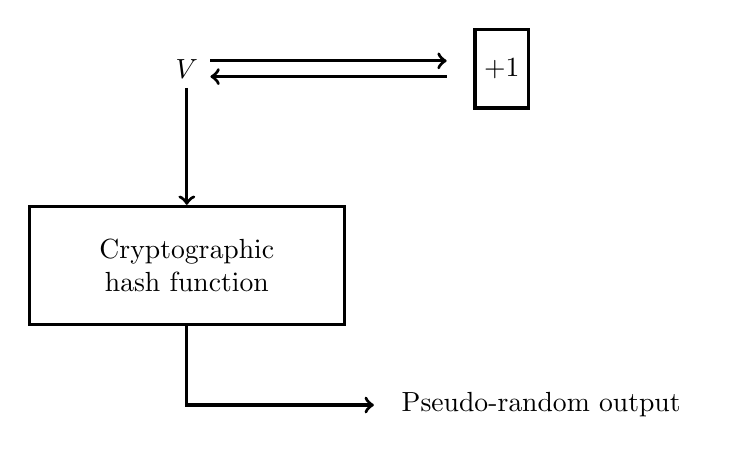
\begin{tikzpicture}
        \draw (0,0) node (V) {$V$};
        \draw[very thick, ->] (0.3,0.1) -- (3.3,0.1);
        \draw[very thick, ->] (3.3,-0.1) -- (0.3,-0.1);
        \draw[very thick] (4,0) node [draw,shape=rectangle,minimum height=1cm] {$+1$};
        \draw[very thick] (V)++(down:2.5cm) node (R1) [draw,shape=rectangle,minimum height=1.5cm,minimum width=4cm,align=center,text width=3cm] {Cryptographic hash function};
        \draw[very thick, ->] (V) -- (R1);
        \draw (R1.south)++(right:4.5cm)++(down:1cm) node (A) [align=center,text width=4cm] {Pseudo-random output};
        \draw[very thick, ->] (R1) |- (A);
    \end{tikzpicture}
    \caption{PRNG using cryptographic hash function}
    \label{fig:1}
\end{figure}

The SP 800-90 specification also provides for periodically updating $V$ to enhance security. The specification also indicates that there are no known or suspected
weaknesses in the hash-based approach for a strong cryptographic hash algorithm, such as SHA-2$^{[1]}$.\\
\\

\subsection{PRNG Based on MAC Function}
In fact, since because HMAC is a widely used standardized MAC function and is implemented in many protocols and applications, HMAC is always used for constructing a MAC-based PRNG rather than the use of a cryptographic hash function for a PRNG. Although HMAC involves two
executions of the underlying hash function for each output block, leading to twice longer execution time, it provides a greater degree of confidence in its security.\\

Here is a figure for PRNG using HMAC:
\begin{figure}[H]
    \centering
    \begin{tikzpicture}
        \draw (0,0) node (V) {$V$};
        \draw[very thick] (V)++(down:2.5cm) node (R1) [draw,shape=rectangle,minimum     height=1.5cm,minimum width=2cm,align=center,text width=2cm] {HMAC};
        \draw[very thick, ->] (V.south) -- (R1);
       \draw (R1.south)++(right:5cm)++(down:1cm) node (A) [align=center,text width=4cm]  {Pseudo-random output};
       \draw[very thick, ->] (R1) |- (A);
        \draw[very thick, ->] (A.west)++(left:0.5cm) |- (V);
        \draw (R1.west)++(left:2cm) node (B) [align=center,text width=4cm] {$K$};
        \draw[very thick, ->] (R1.west)++(left:1.6cm) -- (R1.west);
    \end{tikzpicture}
    \caption{PRNG using HMAC}
    \label{fig:2}
\end{figure}

For the MAC-based approach, there are two inputs: a key $K$ and a seed $V$. Here are some differences among various types of HMAC.\\ \\
For HMAC NIST SP 800-90:
\begin{algorithm}
    \begin{algorithmic}
        \Require \\
        $V$ = seed\\
        $outlen$ = bit length of Hash value\\
        $n$ = desired number of bits for the output
        \Ensure \\
        a random number of $n$ bits
        \Function {RandomGenerator}{$V$, $k$, $seedlen$, $n$, $outlen$}
                \State $m \gets \lceil n/\rm{outlen} \rceil$ 
                \State $w_0 \gets V$ 
                \State $W$ is a null string
                \For {$i=1$ to $m$}  
                    \State $w_i \gets \rm{MAC}(K,w_{i-1})$  
                    \State $W \gets W \mid\mid w_i$  
                \EndFor
                \State \Return{leftmost $n$ bits of $W$}  
        \EndFunction  
    \end{algorithmic}  
\end{algorithm}
\\
\\
\\
For HMAC IEEE 802.11i:
\begin{algorithm}
    \begin{algorithmic}
        \Require \\
        $V$ = seed\\
        $outlen$ = bit length of Hash value\\
        $n$ = desired number of bits for the output
        \Ensure \\
        a random number of $n$ bits
        \Function {RandomGenerator}{$V$, $k$, $seedlen$, $n$, $outlen$}
                \State $m \gets \lceil n/\rm{outlen} \rceil$ 
                \State $W$ is a null string
                \For {$i=1$ to $m$}  
                    \State $w_i \gets \rm{MAC}(K,(V\mid \mid i))$  
                    \State $W \gets W \mid\mid w_i$  
                \EndFor
                \State \Return{leftmost $n$ bits of $W$}  
        \EndFunction  
    \end{algorithmic}  
\end{algorithm}
\\
\\
\\
For HMAC TLS/WTLS:
\begin{algorithm}
    \begin{algorithmic}
        \Require \\
        $V$ = seed\\
        $outlen$ = bit length of Hash value\\
        $n$ = desired number of bits for the output
        \Ensure \\
        a random number of $n$ bits
        \Function {RandomGenerator}{$V$, $k$, $seedlen$, $n$, $outlen$}
                \State $m \gets \lceil n/\rm{outlen} \rceil$ 
                \State $A(0) \gets V$ 
                \State $W$ is a null string
                \For {$i=1$ to $m$}  
                    \State $A(i) \gets \rm{MAC}(K,A(i-1))$
                    \State $w_i \gets \rm{MAC}(K,(A(i)\mid \mid V))$  
                    \State $W \gets W \mid\mid w_i$  
                \EndFor
                \State \Return{leftmost $n$ bits of $W$}  
        \EndFunction  
    \end{algorithmic}  
\end{algorithm}


In HMAC NIST SP 800-90 the combination of $K$ and $V$ form the overall seed for the PRNG. The key remains the same for each block of output, and the data input for each block is equal to the tag output of the previous block. It provides for periodically updating $K$ and $V$ to enhance security.\\


In HMAC IEEE 802.11i, the data input consists of the seed concatenated with a counter. The counter is incremented for each block of output. The security is enhanced comparing to HMAC NIST SP 800-90 since the knowledge of the input and output should not be sufficient to recover $K$ and predict future pseudo-random bits.\\


In HMAC Transport Layer Security protocol and the Wireless Transport Layer Security Protocol abbreviated as TLS/WTLS, for each block of output $w_i$, it invloves invoking HMAC twice. The double use of HMAC doubles the burden, decreases the performance but increases the security overkill.\\


\chapter{  Conclusion and Discussion}
\section{Discussion}

\section{Conclusion}



\chapter{  Bibliography}

\bibliographystyle{plain}
\begin{thebibliography}{0}
\bibitem{1}Hohberger, Horst. "Term Project." 2015. PDF file.
\bibitem{2}Jonathan, Katz; Yehuda, Lindell. "Introduction to Modern Cryptography". 2007. Jonathan Katz and Yehuda Lindell. 
\bibitem{3}Bellare, Mihir; Rogaway, Phillip (21 September 2005). "Introduction". Introduction to Modern Cryptography. p. 10.
\bibitem{4}Menezes, A. J.; van Oorschot, P. C.; Vanstone, S. A. Handbook of Applied Cryptography. ISBN 0-8493-8523-7. Archived from the original on 7 March 2005.
\bibitem{5}William, Stallings. "CRYPTOGRAPHY AND NETWORK SECURITY PRINCIPLES AND PRACTICE". 2011, 2006 Pearson Education, Inc., publishing as Prentice Hall.
\bibitem{6}Alfred J. Menezes, Paul C. van Oorschot, Scott A. Vanstone. "Chapter 9 - Hash Functions and Data Integrity" (PDF). Handbook of Applied Cryptography. p. 361.
\bibitem{7}"Data Origin Authentication". Web Service Security. Microsoft Developer Network.
\bibitem{11}"Cryptanalysis/Signals Analysis". Nsa.gov. 2009-01-15. Retrieved 2013-04-15.
\bibitem{RFC2104} RFC 2104, H. Krawczyk, M. Bellare, R. Canetti, February 1997.

\end{thebibliography}
\end{document}
 
